%%%%%%%%%%%%%%%%%%%%%%%%%%%%%%%%%%%%%%%%%
% Short Sectioned Assignment LaTeX Template Version 1.0 (5/5/12)
% This template has been downloaded from: http://www.LaTeXTemplates.com
% Original author:  Frits Wenneker (http://www.howtotex.com)
% License: CC BY-NC-SA 3.0 (http://creativecommons.org/licenses/by-nc-sa/3.0/)
%%%%%%%%%%%%%%%%%%%%%%%%%%%%%%%%%%%%%%%%%

%----------------------------------------------------------------------------------------
%   PACKAGES AND OTHER DOCUMENT CONFIGURATIONS
%----------------------------------------------------------------------------------------

\documentclass[10pt,a4paper,spanish]{article}

% ---- Entrada y salida de texto -----

\usepackage[spanish]{babel} 
\usepackage[T1]{fontenc} % Use 8-bit encoding that has 256 glyphs
\usepackage[utf8]{inputenc}
\usepackage{cite}
% \usepackage{spreadtab}
% \usepackage{fourier} % Use the Adobe Utopia font for the document - comment this line to return to the LaTeX default
\usepackage[usenames, dvipsnames]{color}
\usepackage[table]{xcolor}
\usepackage{colortbl}
\usepackage[bookmarks=true,colorlinks=true,linkcolor=red,citecolor=blue]{hyperref}
% \usepackage{cite}
% \usepackage[official]{eurosym}
\usepackage{tikz}
% \usepackage{pgfplots}
% \pgfplotsset{compat=1.5}

% \usepackage{subfigure}

\usepackage{pseudocode}

% ---- Otros paquetes ----
\usepackage{enumerate}
\usepackage{amsmath,amsfonts,amsthm,amssymb} % Math packages
\usepackage{graphics,graphicx} %para incluir imágenes y notas en las imágenes
% Para hacer tablas comlejas
%\usepackage{multirow}
%\usepackage{threeparttable}

\usepackage[a4paper, margin=1.3in]{geometry}


\usepackage{sectsty} % Allows customizing section commands
\allsectionsfont{\centering \normalfont\bfseries\scshape} % Make all sections centered, the default font and small caps
\usepackage{fancyhdr}
\pagestyle{fancy}
%con esto nos aseguramos de que las cabeceras de capítulo y de sección vayan en minúsculas

\renewcommand{\sectionmark}[1]{%
      \markright{\thesection\ #1}}
\fancyhf{} %borra cabecera y pie actuales
\fancyhead[LE,RO]{{\bfseries Práctica 1}}
\fancyhead[LO]{\bfseries Marta Gómez}
\fancyfoot[C]{\thepage{}}
\renewcommand{\headrulewidth}{0.5pt}
\renewcommand{\footrulewidth}{0pt}
\addtolength{\headheight}{0.5pt} %espacio para la raya
\fancypagestyle{plain}{%
      \fancyhead{} %elimina cabeceras en páginas "plain"
      \renewcommand{\headrulewidth}{0pt} %así como la raya
}

\numberwithin{equation}{section} % Number equations within sections (i.e. 1.1, 1.2, 2.1, 2.2 instead of 1, 2, 3, 4)
\numberwithin{figure}{section} % Number figures within sections (i.e. 1.1, 1.2, 2.1, 2.2 instead of 1, 2, 3, 4)
\numberwithin{table}{section} % Number tables within sections (i.e. 1.1, 1.2, 2.1, 2.2 instead of 1, 2, 3, 4)

\setlength\parindent{0pt} % Removes all indentation from paragraphs - comment this line for an assignment with lots of text
\setlength{\parskip}{1ex plus 0.5ex minus 0.2ex}

\newcommand{\horrule}[1]{\rule{\linewidth}{#1}} % Create horizontal rule command with 1 argument of height

%----------------------------------------------------------------------------------------
%   TÍTULO Y DATOS DEL ALUMNO
%----------------------------------------------------------------------------------------

\title{
\normalfont \normalsize 
{\bf Redes y Sistemas Complejos} \\ Curso 2015-2016 \\ [25pt] % Your university, school and/or department name(s)
\horrule{0.5pt} \\[0.4cm] % Thin top horizontal rule
\huge \textsc{Práctica 1: \\ Análisis Preliminar y Visualización \\ Básica de una red de Facebook \\ con \textit{Gephi}} \\ % The assignment title
\horrule{2pt} \\[0.5cm] % Thick bottom horizontal rule
}

\author{\textit{Marta Gómez Macías}} %\\ \texttt{mgmacias95@correo.ugr.es} \\ 75929776Z \\[0.5cm]

% \date{\normalsize\today} % Incluye la fecha actual

% \usepackage{pdflscape}

%----------------------------------------------------------------------------------------
% DOCUMENTO
%----------------------------------------------------------------------------------------

\begin{document}
%Cambiar Cuadros por Tablas y lista de...
\renewcommand{\listtablename}{Índice de tablas}
\renewcommand{\tablename}{Tabla} 

\begin{titlepage}
\begin{center}

\includegraphics[width=0.2\textwidth]{ugr}

\normalfont \normalsize 
{\bf Redes y Sistemas Complejos} \\ Curso 2015-2016 \\ [25pt] % Your university, school and/or department name(s)
\horrule{0.5pt} \\[0.4cm] % Thin top horizontal rule
{\huge \textsc{Práctica 1: \\ Análisis Preliminar y Visualización \\ Básica de una red de Facebook \\ con \textit{Gephi} \\}} % The assignment title
\horrule{2pt} \\[0.5cm] % Thick bottom horizontal rule

{\Large \textit{Marta Gómez Macías} \\ \texttt{mgmacias95@correo.ugr.es} \\ 75929776Z \\[0.5cm]

\date{\today}} % Incluye la fecha actual
\end{center}
\end{titlepage}

\tableofcontents % para generar el índice de contenidos

% \listoffigures

% \listoftables

\section{Descripción de la red}

La red a analizar ha sido extraída del grupo de \textit{Facebook} llamado \href{https://www.facebook.com/groups/bastadeabusosconnuestrasfotos/}{\textbf{STOP CLAUSULAS ABUSIVAS A LOS FOTÓGRAFOS}}.

\subsection{Grafo de la red}

En la \hyperref[completo]{Figura \ref*{completo}} vemos una representación del grafo completo de la red y en la \hyperref[conexa]{Figura \ref*{conexa}}, una representación de la componente gigante. Ambas son prácticamente iguales, salvo por dos nodos que están conectados entre sí más alejados del resto. 

A simple vista, se ve que hay dos usuarios que participan muchísimo en todos los posts del grupo. Después vemos nodos con tamaño medio, que supongo que corresponden con los usuarios que han publicado un post y muchos nodos conectados a estos, que corresponden con los usuarios que iteraccionan con ese post.

Para generar la visualización he optado finalmente por el algoritmo de visualización \textbf{Yifan Hu}, con los parámetros que trae por defecto. El \textbf{tamaño} de los nodos ha sido calculado por su \textbf{grado}. A la hora de \textbf{colorear} los nodos, he usado un atributo de los datos llamado \textbf{made\_posts} que mide el número de posts que ha hecho ese usuario. Con este coloreado confirmo lo que digo en el párrafo anterior: los nodos con mayor grado corresponden con los usuarios que han hecho algún post y los nodos con un grado pequeño, con los usuarios que interaccionan con dicho post. En la \hyperref[proporcion]{Figura \ref*{proporcion}}, vemos la proporción de usuarios según el número de posts que han escrito. El usuario que más posts ha escrito se ha coloreado en azul (se sitúa en el centro del grafo) y los dos usuarios con mayor grado, han escrito dos posts pero han iteractuado más con el resto de usuarios. Los nodos coloreados en morado son los que no han escrito ningún post, y representan la mayoría.

\begin{figure}[!h]
    \centering
    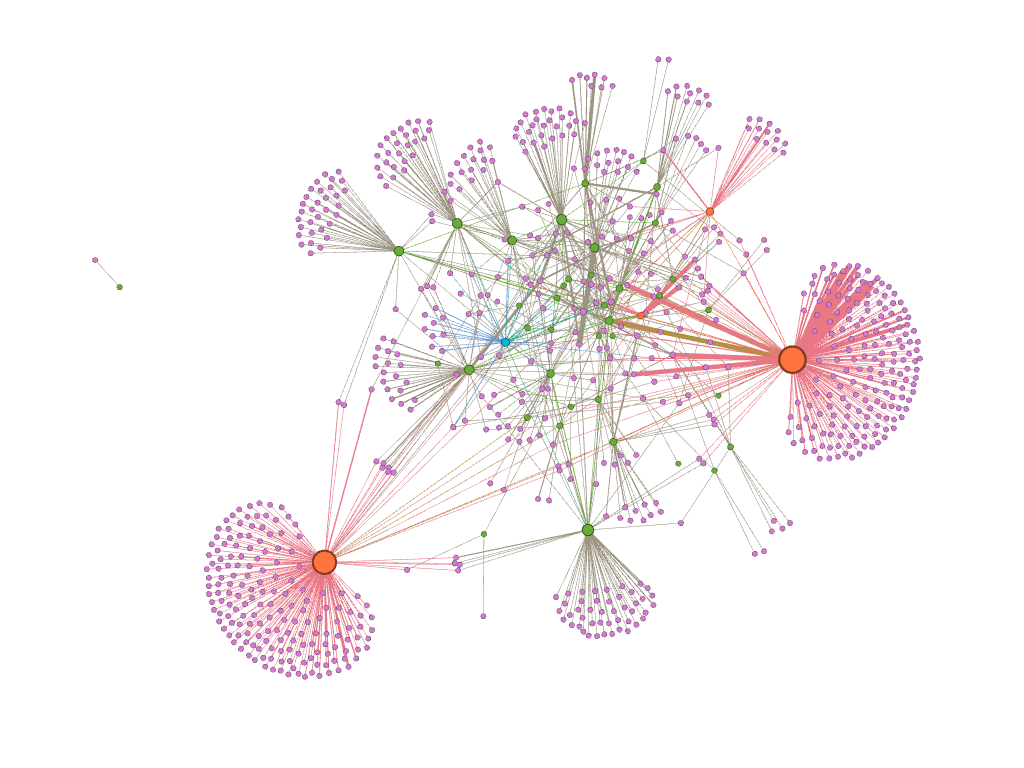
\includegraphics[width=\textwidth]{1}
    \caption{Representación del grafo completo de la red}
    \label{completo}
\end{figure}

\begin{figure}[!h]
    \centering
    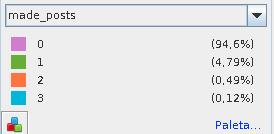
\includegraphics[width=0.5\textwidth]{3}
    \caption{Proporción de nodos según el número de posts que han hecho.}
    \label{proporcion}
\end{figure}

\begin{figure}[!h]
    \centering
    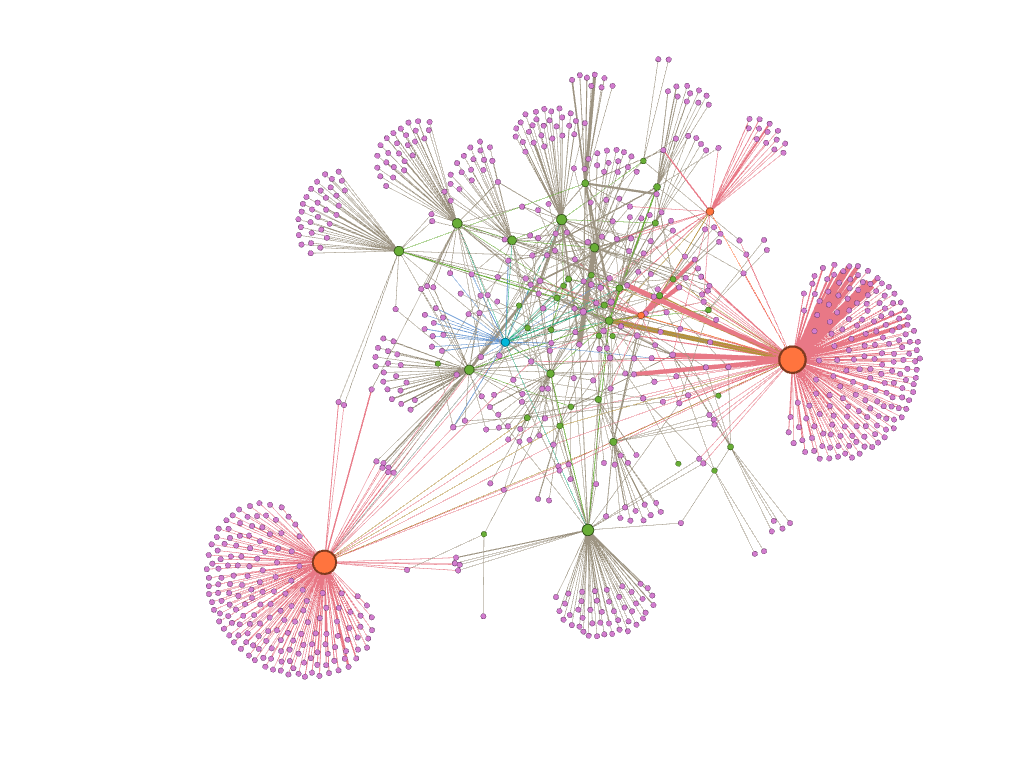
\includegraphics[width=\textwidth]{2}
    \caption{Representación de la componente gigante del grafo de la red}
    \label{conexa}
\end{figure}

\section{Datos estadísticos sobre la red}

En la \hyperref[tabla]{Tabla \ref*{tabla}} vemos una serie de datos estadísticos sobre la red. 

Viendo el número máximo de enlaces, ya sabemos que el grafo \textbf{no es completo}, ya que $L_{max} > L$. Además, teniendo en cuenta que la densidad del grafo es $d = 0.003$, vemos que además de no ser completo \textbf{hay poca interconexión} entre los nodos: hay nodos que reciben muchas interacciones y otros que sólo interactúan con un único nodo, es decir, hay pocos nodos que publiquen posts pero muchos que comentan e interactúan con los distintos posts. Podemos comprobar estas dos afirmaciones observando el grafo (\hyperref[completo]{Figura \ref*{completo}}). 

Si observamos el grado medio, podemos concluir que, en media, \textbf{cada usuario interactúa con unos 2 posts}.

\begin{table}[!h]
\centering
\begin{tabular}{| c | c |}
\hline
Número de nodos ($N$) & $815$ \\
\hline
Número de enlaces ($L$) & $1075$ \\
\hline
Número máximo de enlaces ($L_{max}$) & $331705$ \\
\hline
Densidad del grafo ($\frac{L}{L_{max}}$) & $0.003$ \\
\hline
Grado medio ($<k>$) & $2.683$ \\
\hline
Diámetro ($d_{max}$) & $6$ \\
\hline
Distancia media ($d$) & $3.543$ \\
\hline
Coeficiente medio de clustering ($<C>$) & $0.105$ \\
\hline
Número de componentes conexas & $2$ \\
\hline
Número de nodos de la componente gigante & $813$ ($99.75\%$)\\
\hline
Número de aristas de la componente gigante & $1074$ ($99.91\%$)\\
\hline
\end{tabular}
\caption{Datos estadísticos sobre la red}
\label{tabla}
\end{table}

\section{Gráficos de distribuciones de la red}

\end{document}